% !TeX spellcheck = cs_CZ
%{\tikzset{external/prefix={tikz/FYZII/}}
% \tikzset{external/figure name/.add={ch11_}{}}
%---------------------------------------------------------------------------------------------------
% file fey2ch11.tex
%---------------------------------------------------------------------------------------------------
%=========================== Kapitola: Vnitřní stavba dielektrik ===================================
\setchaptertoc
\chapter{Vnitřní stavba dielektrik}\label{fyz:IIchapXI}

  \section{Molekulové dipóly}\label{fyz:IIchapXIsecI}
  \section{Elektronová polarizace}\label{fyz:IIchapXIsecII}
  \section{Polární molekuly. Orientační polarizace}\label{fyz:IIchapXIsecIII}
  \section{Elektrické pole v dutinách dielektrika}\label{fyz:IIchapXIsecIV}
  \section{Permitivita kapalin. Clausiova-Mosottiova rovnice}\label{fyz:IIchapXIsecV}
  \section{Pevná dielektrika}\label{fyz:IIchapXIsecVI}
  \section{Feroelektřina. BaTiO3}\label{fyz:IIchapXIsecVII}
  \section{Příklady a cvičení}\label{fyz:IIchapXIsecVIII}

    \begin{figure}[ht!]
      \centering
      \subcaptionbox{\label{fyz:fig0714a}}{\luafigure[0.65]{fyz_fig0714a.pdf}}               \\
      \subcaptionbox{\label{fyz:fig0714b}}{\luafigure[0.65]{fyz_fig0714b.pdf}}
      \label{fyz:fig0714}
      \caption{
               (\cite[s.~748]{Feynman02})}
    \end{figure}

    \begin{figure}[ht!]
      \centering
      \subcaptionbox{\label{fyz:fig0715a}}{\luafigure[0.45]{fyz_fig0715a.pdf}}
      \subcaptionbox{\label{fyz:fig0715b}}{\luafigure[0.45]{fyz_fig0715b.pdf}}
      \label{fyz:fig0715}
      \caption{
               (\cite[s.~748]{Feynman02})}
    \end{figure}

    \begin{figure}[ht!] %\ref{fyz:fig0716}
      \centering
      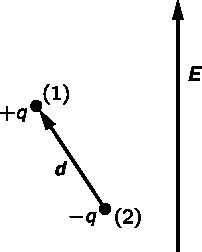
\includegraphics[width=0.4\linewidth]{fyz_fig0716.pdf}
      \caption{
               (\cite[s.~707]{Feynman02})}
      \label{fyz:fig0716}
    \end{figure}

    \begin{figure}[ht!] %\ref{fyz:fig0717}
      \centering
      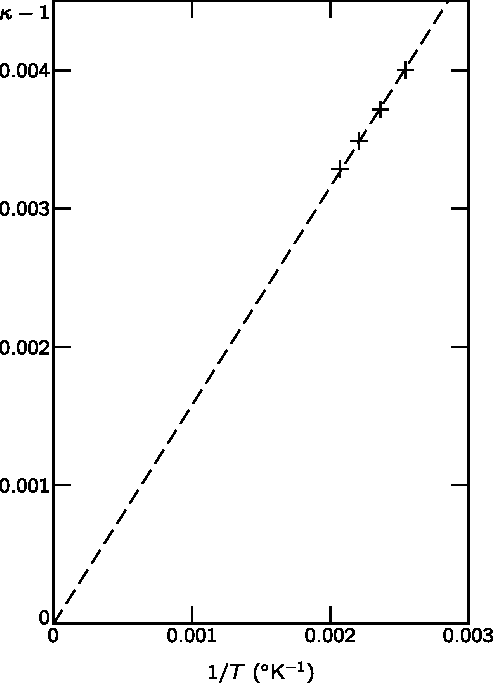
\includegraphics[width=0.5\linewidth]{fyz_fig0717.pdf}
      \caption{
               (\cite[s.~707]{Feynman02})}
      \label{fyz:fig0717}
    \end{figure}

    \begin{figure}[ht!] %\ref{fyz:fig0718}
      \centering
      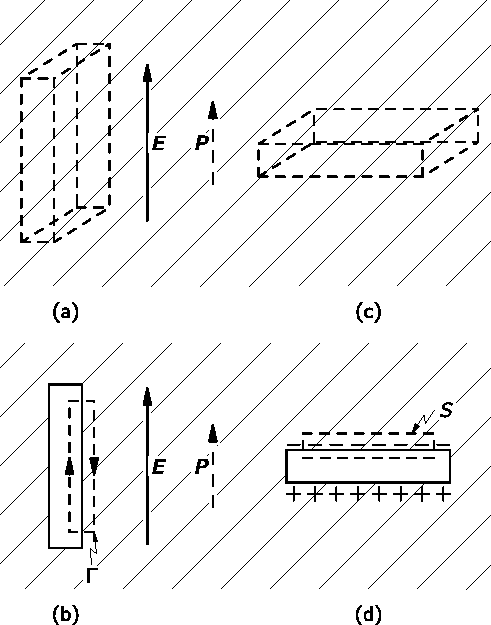
\includegraphics[width=0.5\linewidth]{fyz_fig0718.pdf}
      \caption{
               (\cite[s.~707]{Feynman02})}
      \label{fyz:fig0718}
    \end{figure}

    \begin{figure}[ht!] %\ref{fyz:fig0719}
      \centering
      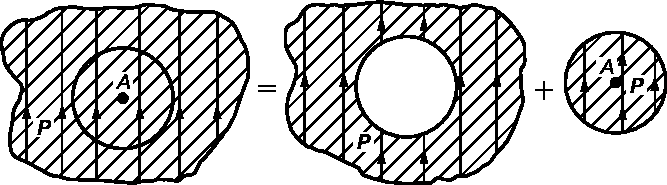
\includegraphics[width=0.5\linewidth]{fyz_fig0719.pdf}
      \caption{
               (\cite[s.~707]{Feynman02})}
      \label{fyz:fig0719}
    \end{figure}

    \begin{figure}[ht!] %\ref{fyz:fig0720}
      \centering
      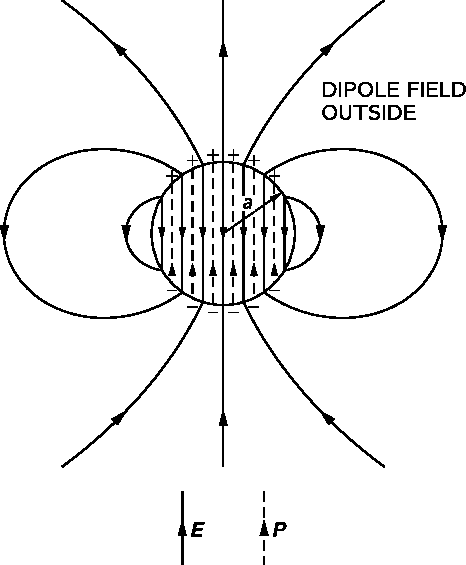
\includegraphics[width=0.5\linewidth]{fyz_fig0720.pdf}
      \caption{
               (\cite[s.~707]{Feynman02})}
      \label{fyz:fig0720}
    \end{figure}

    \begin{figure}[ht!] %\ref{fyz:fig0721}
      \centering
      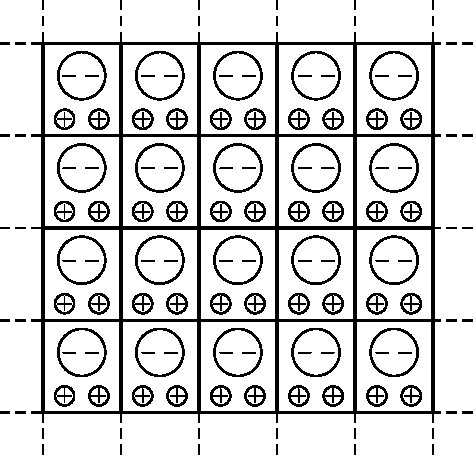
\includegraphics[width=0.5\linewidth]{fyz_fig0721.pdf}
      \caption{
               (\cite[s.~707]{Feynman02})}
      \label{fyz:fig0721}
    \end{figure}

    \begin{figure}[ht!] %\ref{fyz:fig0722}
      \centering
      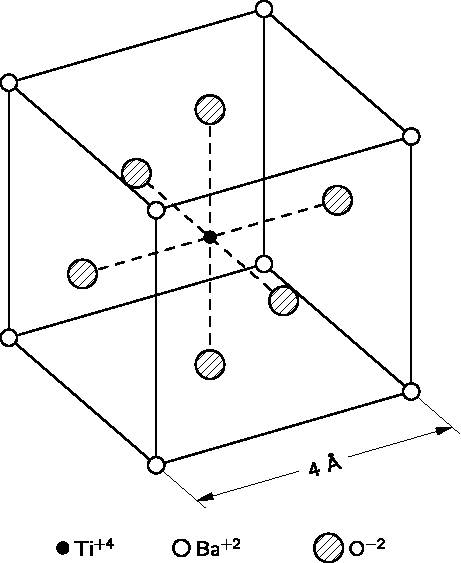
\includegraphics[width=0.5\linewidth]{fyz_fig0722.pdf}
      \caption{
               (\cite[s.~707]{Feynman02})}
      \label{fyz:fig0722}
    \end{figure}

    \begin{figure}[ht!] %\ref{fyz:fig0723}
      \centering
      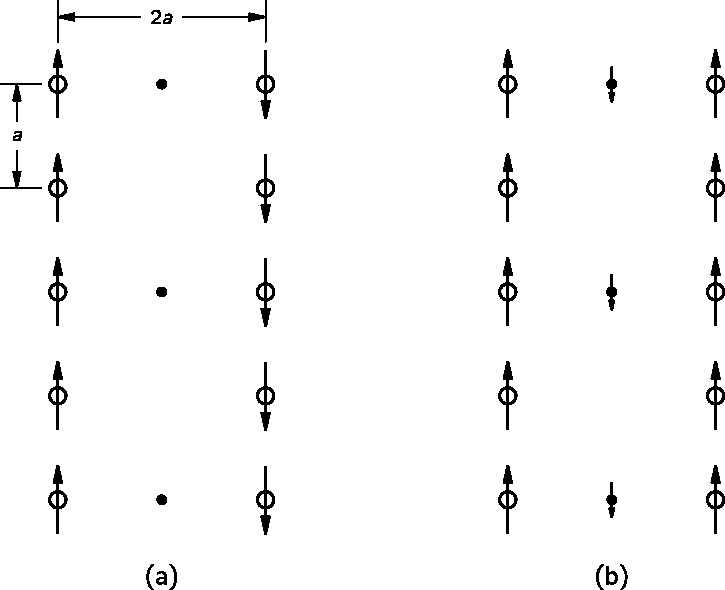
\includegraphics[width=0.7\linewidth]{fyz_fig0723.pdf}
      \caption{
               (\cite[s.~707]{Feynman02})}
      \label{fyz:fig0723}
    \end{figure}

\todo[inline]{Kapitola fey2ch11 je nedodělaná, obsahuje pouze obrázky}
%} %tikzset
%---------------------------------------------------------------------------------------------------
